\chapter{Dataset}\label{chapter:Dataset}

\section{Scope and Design}
The main goal is to gather a diverse and high-quality dataset which represents static
real-world HTML/CSS webpages. The dataset should (1) include multiple domains and layouts,
(2) contain annotated accessibility violations and (3) has a reasonable size to be
statistically relevant, but is also small enough to be analyzed manually.
There is no publicly available dataset which fullfills all requirements.

\section{Construction}
Two promising examples in the field of Image-to-Code are \textit{Design2Code}~\parencite{si2024design2code} 
and \textit{Webcode2m}~\parencite{gui2024webcode2m}. 
Both have used existing, large datasets and applied different processing steps to 
filter bad examples and remove noise or redundancy from the code. Based on their
dataset curation, both serve as a good base for this thesis.\newline
Therefore, we decided to use both datasets and manually select 53 high-quality data 
entries. Those 53 data entries consist of 28 entries from \textit{Design2Code} and 25 entries
from \textit{Webcode2m}. In order to compare them on a fair basis, we only collect webpages 
that have english as their primary language.

\subsection{Content Distribution}
By using data entries of various domains and different layouts, we make sure to get 
a fair representation of the distribution of webpages in the real world. Based on 
our manual selection, we present the domain distribution in a pie chart in Figure 1.

\begin{figure*}[p]
  \centering
  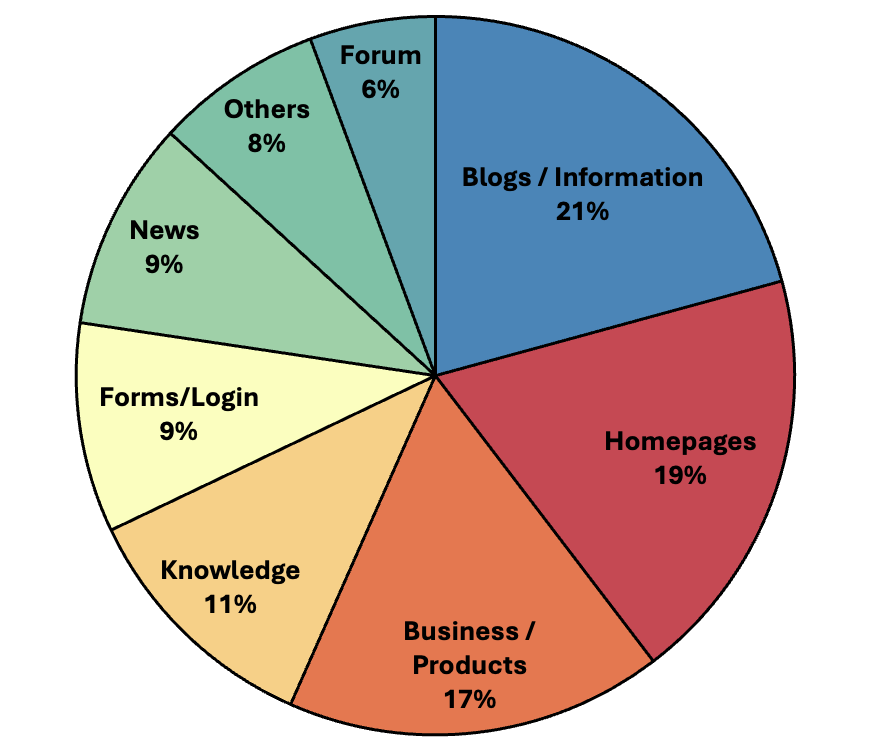
\includegraphics[width=\textwidth]{figures/dataset_distribution.png}
  \caption{Distribution of Topics in Dataset}
  \label{fig:dataset_distribution}
\end{figure*}

\section{Dataset Alignment}
Due to the fact that Design2Code and Webcode2m use different strategies to purify
their data, it is necessary to align both datasets.
This includes (1) removing all external dependencies such as multimedia files (images, 
audio, videos, links), replacing them with placeholders such as src="placeholder.jpg" 
for images or href="\#" for <a> Tags. Furthermore, (2) scripts and other dynamic 
contents are neutralised.
Lastly, (3) non-visible content, such as advertisement-related tags or hidden elements 
are removed, because they are not required in an Image-to-Code environment and 
could possibly bias the accessibility score negatively.


\section{Data Leakage}
In a last step we try to rule out the risk of data leakage. Both datasets have been
published on Huggingface within three months of the official knowledge-cutoff 
of \textit{GPT-4o} and \textit{Gemini flash 2.0}.
This means that theoretically both datasets could have been part of the LLMs' training
data.
Therefore, we create a 
new, leakage-proof dataset of 20 entries which we test the LLMs on and compare their 
performance.
This test dataset has 20 data entries and we construct it as follows:

\begin{itemize}
  \item \textbf{Mutation of existing Data Entries:} We use 10 randomly-selected data entries of our existing 
  dataset. Each data entry has been (1) rewritten by an LLM. While the meaning
    and the length (max ±20 \%) remains roughly the same, the wording changes
    completely. The text appearance (2) is further changed by a set of 5 commonly used fonts in webpages and 
    by changing (3) the \textit{HUE} color code of each element slightly based on a random shift (±20 degrees). \newline
    Additionally, we randomly change (4) the structure of the data entries manually. Structural 
    blocks, such as headers, tables and images, are shuffled within and across different 
    pages. This ensures a completely new layout, while making sure that the new data entries 
    remain realistic and similar to their real-world origin.

  \item \textbf{Collection of new Data Entries:} The other 10 data entries have been crawled from 
    two Github repositories created in 2025. \textit{AlphaOneLabs}~\parencite{alphaonelabs_education} is an educational project 
    with different webpage styles and layouts. The second repository \textit{E-Commerce-Site}~\parencite{nuranferhan_ecommerce}
    offers a wide range of e-commerce related webpages. On this basis, we 
    randomly sample 10 diverse webpages.
\end{itemize}


\subsection{Results}
Across all prompting techniques, \textit{GPT-4o} and \textit{Gemini flash 2.0} 
performed better on the 
\textit{leakage-test split} than on the original dataset in terms of their final scores.
Since the results do not show any statistically significant drop in performance, we 
do not have any evidence for data leakage and assume that the LLMs have not seen the existing 
data. We proceed with the full dataset in the following experiments.


